\documentclass[tikz]{standalone}
\usepackage{pgfplots}
\pgfplotsset{compat=1.15}
\usepackage{mathrsfs}
\usetikzlibrary{arrows,calc}
\usepackage{tkz-euclide}

\pagestyle{empty}

\definecolor{AngleClr}{rgb}{0,0.39215686274509803,0}
\definecolor{ShapeClr}{rgb}{0.6,0.2,0}

\begin{document}

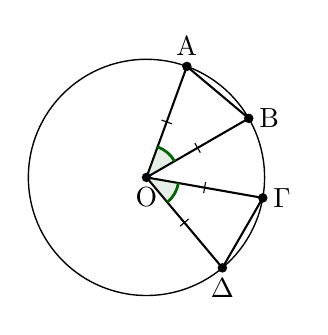
\begin{tikzpicture}[scale=.75]
\tkzSetUpLine[line width=1pt,color=black]
\tkzSetUpPoint[fill=black]

\tkzDefPoints{0/0/O,2/0/X}

\tkzDefPoint(30:2){B}
\tkzDefPoint(70:2){A}
\tkzDefPoint(-10:2){C}
\tkzDefPoint(-50:2){D}

\tkzDrawSegments[line width=0.75pt,color=black](O,A O,B O,C O,D A,B C,D)

\tkzDrawCircle[color=black,line width=0.5pt](O,X)

\tkzFillAngles[fill=AngleClr,size=.55,fill opacity=0.1](B,O,A D,O,C)
\tkzMarkAngles[line width=1pt,size=.55,color=AngleClr](B,O,A D,O,C)

\tkzDrawPoints[size=3](A,B,O,C,D)
\tkzLabelPoint[above](A){$\rm A$}
\tkzLabelPoint[right](B){$\rm B$}
\tkzLabelPoint[right](C){$\rm \Gamma$}
\tkzLabelPoint[below](D){$\rm \Delta$}
\tkzLabelPoint[below](O){$\rm O$}

\tkzMarkSegments[mark=|,size=2](O,A O,B O,C O,D)

\end{tikzpicture}
\end{document}
